% 12-module course roadmap. Edit this file (not the .svg) and rerun
% tools/build-diagrams.sh to regenerate.
\documentclass[tikz,border=4pt]{standalone}
\usepackage{tikz}
\usetikzlibrary{positioning,fit,decorations.pathreplacing,calligraphy}
\definecolor{fpfill}{HTML}{E8F0E6}
\definecolor{fpedge}{HTML}{3A6C52}
\definecolor{secfill}{HTML}{FBEED2}
\definecolor{secedge}{HTML}{B97A18}
\definecolor{labelgrey}{HTML}{444444}
\begin{document}
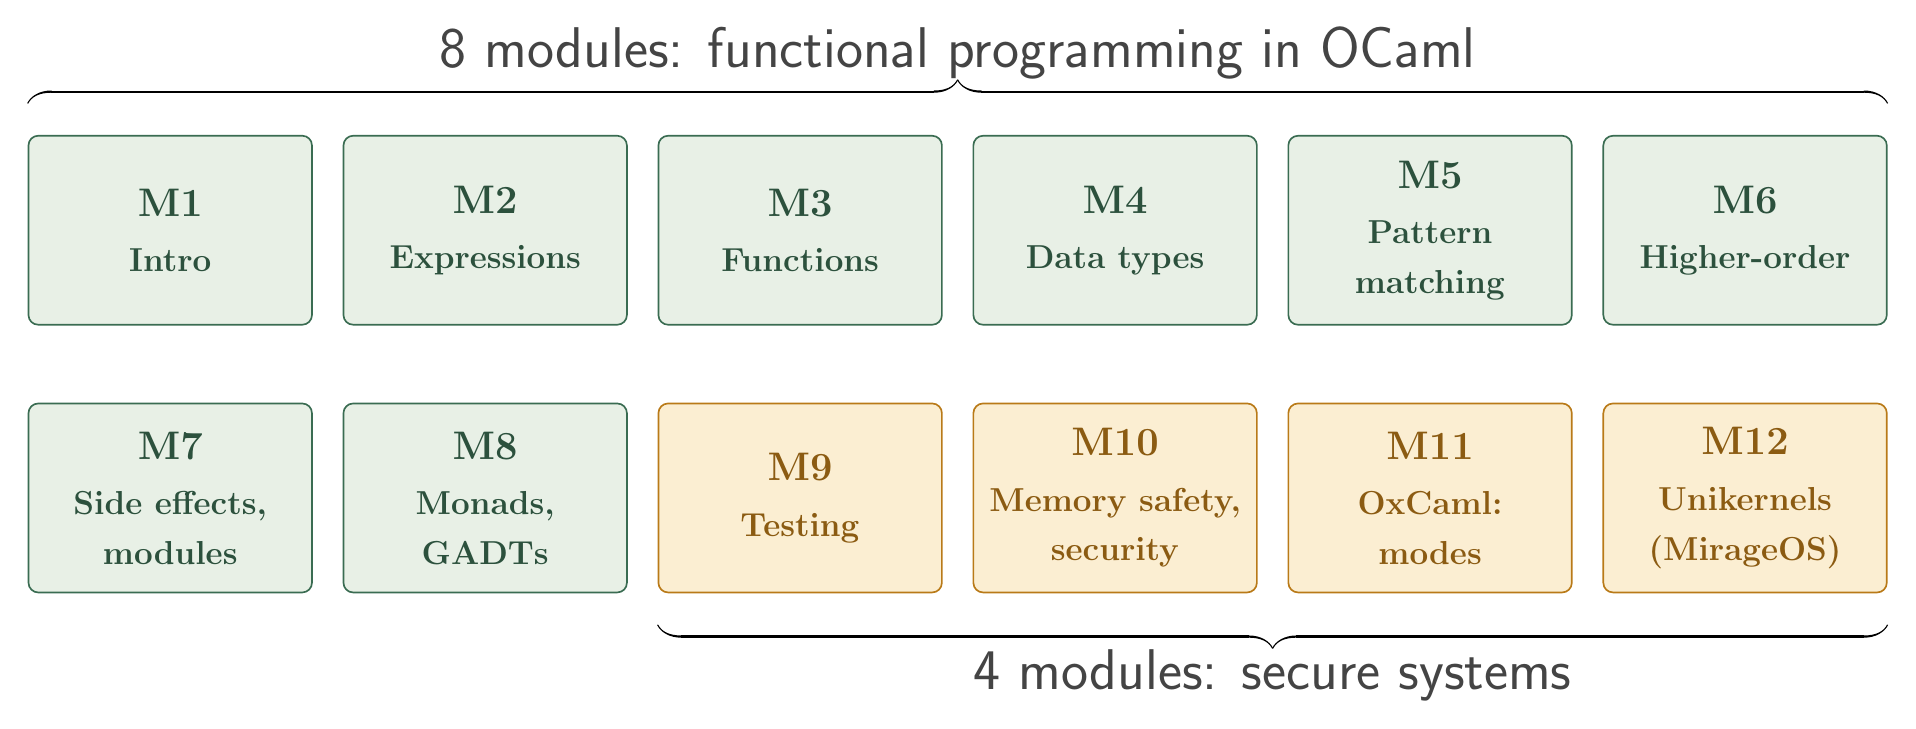
\begin{tikzpicture}[
  font=\sffamily,
  every node/.style={inner sep=0pt},
  tile/.style={
    rounded corners=3.5pt,
    minimum width=36mm, minimum height=24mm,
    align=center, line width=0.6pt,
    font=\Large
  },
  fp/.style={tile, fill=fpfill, draw=fpedge, text=fpedge!75!black},
  sec/.style={tile, fill=secfill, draw=secedge, text=secedge!75!black},
  bracket/.style={decorate, decoration={calligraphic brace, raise=2mm, amplitude=3mm}, draw=labelgrey!80, line width=0.8pt},
  x=40mm, y=-34mm
]

% Row 1 (y = 0): M1 .. M6, all FP
\node[fp] (m1)  at (0,0)  {\textbf{M1}\\[2pt]\large\textbf{Intro}};
\node[fp] (m2)  at (1,0)  {\textbf{M2}\\[2pt]\large\textbf{Expressions}};
\node[fp] (m3)  at (2,0)  {\textbf{M3}\\[2pt]\large\textbf{Functions}};
\node[fp] (m4)  at (3,0)  {\textbf{M4}\\[2pt]\large\textbf{Data types}};
\node[fp] (m5)  at (4,0)  {\textbf{M5}\\[2pt]\large\textbf{Pattern}\\\large\textbf{matching}};
\node[fp] (m6)  at (5,0)  {\textbf{M6}\\[2pt]\large\textbf{Higher-order}};

% Row 2 (y = 1): M7, M8 (FP) under M1, M2; then M9..M12 (secure) under M3..M6
\node[fp]  (m7)  at (0,1)  {\textbf{M7}\\[2pt]\large\textbf{Side effects,}\\\large\textbf{modules}};
\node[fp]  (m8)  at (1,1)  {\textbf{M8}\\[2pt]\large\textbf{Monads,}\\\large\textbf{GADTs}};
\node[sec] (m9)  at (2,1) {\textbf{M9}\\[2pt]\large\textbf{Testing}};
\node[sec] (m10) at (3,1) {\textbf{M10}\\[2pt]\large\textbf{Memory safety,}\\\large\textbf{security}};
\node[sec] (m11) at (4,1) {\textbf{M11}\\[2pt]\large\textbf{OxCaml:}\\\large\textbf{modes}};
\node[sec] (m12) at (5,1) {\textbf{M12}\\[2pt]\large\textbf{Unikernels}\\\large\textbf{(MirageOS)}};

% Bracket above row 1, labelling all FP modules
\draw[bracket] ([yshift=2mm]m1.north west) -- ([yshift=2mm]m6.north east)
  node[midway, above=5mm, color=labelgrey] {\huge 8 modules: functional programming in OCaml};

% Smaller bracket below the row 2 secure-systems tiles
\draw[bracket, decoration={calligraphic brace, raise=2mm, amplitude=3mm, mirror}]
  ([yshift=-2mm]m9.south west) -- ([yshift=-2mm]m12.south east)
  node[midway, below=5mm, color=labelgrey] {\huge 4 modules: secure systems};

\end{tikzpicture}
\end{document}
